\chapter{Testovanie}
Testovanie programu, a to predovšetkým funkčnosti jednotlivých YAML modulov prebiehalo postupne pri ich zostavovaní. Funkčnosť jednotlivých metód a funkcií bola testovaná rôznymi priaznivými, ako aj chybovými vstupmi, ktoré by mohli nastať zlým nastavením programu, ale aj nekonzistentným vstupom. Pre testovanie YAML modulov bolo nevyhnutné získať čo najviac kombinácií nastavení, na čo bol použitý program GNS3, ktorý dokáže simulovať sieťové zariadenia a vyexportované nastavenia týchto zariadení môžu byť následne testované. Ako už bolo spomenuté v prechádzajúcich kapitolách, tak na vyhľadávanie nedostatkov boli použité regulárne výrazy. Dĺžka týchto regulárnych výrazov v tomto programe je od pár desiatkov znakov až po cca. 1500 pri komplikovanom filtračnom pravidle. Niekedy na prvý pohľad komplikované regulárne výrazy sú nutné, pretože zápis niektorých príkazov má množstvo variácií či už v poradí jednotlivých častí, alebo rozdielnej syntaxe naprieč verziami operačného systému. Validácia a ladenie regulárnych výrazov  prebiehala za pomoci stránky \url{www.regex101.com}. Na validáciu bolo nutné mnohokrát rôznym spôsobom nakombinovať časti príkazu a taktiež vytvoriť zdanlivo fungujúci príkaz, v ktorom sa nemohla nájsť zhoda.  

\section{Testovacie prostredie}
\begin{table}[H]
	\begin{tabular}{l|l}
		CPU:        & Intel Core i5 6200U                                            \\
		RAM:        & 12 GB                                                          \\
		OS:         & Debian 10 (Buster)                                             \\
		Python:     & 3.7.3                                                          \\
		Knižnice:   & ruamel.yaml 0.16.10, pdfkit 0.6.1                              \\
		SW:         & GNS3 2.1.21, wkhtmltopdf 0.12.5                                \\
		Sieťový HW: & Cisco IOU L2 15.2d, Cisco IOU L3 15.5(2)T, Cisco IOSvL2 15.2.1
	\end{tabular}
	\caption{Testovacie prostredie}
	\label{tab:test_conf}
\end{table}
 

\section{Príklad spustenia so vzorovými nastaveniami}
Pre otestovanie a demonštráciu funkčnosti výsledného programu bola v nástroji GNS3 vytvorená topológia a následne vyexportované nastavenia jednotlivých sieťových prvkov. Tieto nastavenia dostupné v \texttt{init\_configs/topologia\_diplomova\_praca} budú použité v nasledujúcom návode na demonštračné spustenie. Vyexportované nastavenia obsahujú zámerne chyby, aby bolo možné otestovať jednak vyhľadávanie nedostatkov v nastaveniach, ale aj úspešnosť aplikovania generovaných náprav. Úspešnosť aplikovaných náprav bude verifikovaná opätovným spustením programu, no s vyexportovanými konfiguráciami po aplikácií nápravných príkazov. Pri spúšťaní je treba byť v zložke s hlavným skriptom \texttt{netsec.py} a spúšťať ho z tohto umiestnenia. V prípade použitia nastavení z testovacej konfigurácie stačí použiť nasledujúci príkaz nižšie. Pri analýze iných nastavení je nutné vytvoriť novú zložku v \texttt{init\_configs} napríklad \texttt{topológia\_FEKT\_VUT} a do nej umiestniť vyexportované konfigurácie. Viac o tejto problematike v \ref{popis_fungovania}. Keďže kvôli časovej náročnosti je doposiaľ prítomná podpora iba pre zariadenia Cisco s operačným systémom IOS, tak je jedinou možnosťou špecifikovať prepínače s nasledujúcimi argumentami \texttt{---vendor ``cisco`` ---os ``ios``}. Pri opätovnom spustení prvotnej analýzy, teda zistení základných informácií o zariadeniach, nie samotnom vyhľadávaní nedostatkov, je občas žiadúce ponechať v minulosti vyplnené premenné v \texttt{own\_variables.yaml} z predchádzajúceho spustenia programu. Toto sa vykonáva pomocou prepínaču \texttt{---keep-own-vars}. Každá časť spustenia obsahuje ukazateľa postupu v percentách, aby bolo zrejmé, že program niečo vykonáva, podrobnejšie výpisy nie sú prítomné, pretože by samostatné nadmerné vypisovanie mohlo spomaľovať beh programu. Po poslednom sprocesovanom zariadení sa za ukazateľom ukáže namiesto percent hlásenie \texttt{Done!}. Pri opätovnom spustení programu s argumentom \texttt{analyze} sa predchádzajúce zistenia, správy, moduly s informáciami automaticky presunú do umiestnenia \texttt{old\_configs/topologia\_diplomova\_praca}, kde sa vytvorí vždy zložka s aktuálnym časom.

\begin{minipage}{\linewidth}		
	\begin{lstlisting}[frame=single,numbers=right,caption={Spustenie úvodnej analýzy topológie},label=lst:netsec_analyze,basicstyle=\ttfamily\footnotesize, keywordstyle=\color{black}\bfseries\underbar,language=,breaklines=true]
	./netsec.py analyze --workspace "topologia_diplomova_praca" 
	  --vendor "cisco" --os "ios"
	
	[========] Done!
	
	Hostname                      Facility layer(Automatically set)
	Access_SW1                    access
	Access_SW2                    access
	Access_SW3                    access
	BRANCH_Office                 collapsed_all
	Core                          core
	Dist_Router                   distribution
	Dist_SW1                      distribution
	Dist_SW2                      collapsed_distribution_access
	
	To edit facility layer go to diplomova_praca/src/device_configs/
	topologia_diplomova_praca to corresponding folder named 
	by hostname and change variable 'faciliy_layer' in 
	device_info.yaml
	
	Workspace successfully analyzed!
	\end{lstlisting}
\end{minipage}
\newpage
\vspace{2em}
V ďalšej fáze sa spúšťa vyhľadávanie a generovanie náprav nájdených nedostatkov, pokiaľ je to možné. Ešte pred tým je však nutné v aktuálnom workspace, teda v \texttt{device\_configs/topologia\_diplomova\_praca} vyplniť východzie nastavenia premenných v súbore \texttt{own\_variables.yaml}. Pre urýchlenie je takýto súbor predvyplnený v zložke \texttt{testing} a stačí ho nakopírovať a prepísať v adresári\\ \texttt{device\_configs/topologia\_diplomova\_praca}. V prípade nejakej nevyplnenej premennej v tomto súbore je administrátor notifikovaný a musí potvrdiť, že nevyplnením premenných nemusí generovanie nápravy fungovať ako má. Z dôvodu anonymizácie je možné neukladať úspešné nájdenia a v následne vygenerovanej správe informovať iba o prítomnosti a neprítomnosti nastavenia pomocou prepínača \texttt{---hide-match}.

\begin{minipage}{\linewidth}		
	\begin{lstlisting}[frame=single,numbers=right,caption={Spustenie vyhľadávania nedostatkov a generovania nápravy},label=lst:netsec_audit,basicstyle=\ttfamily\footnotesize, keywordstyle=\color{black}\bfseries\underbar,language=,breaklines=true]
	./netsec.py audit-check --workspace "topologia_diplomova_praca"
	
    [========] Done!
    
    Audit check was done on workspace!
	\end{lstlisting}
\end{minipage}

\vspace{2em}
Následne sa môže spustiť vygenerovanie záverečných správ pre každé zariadenie. Z dôvodu anonymizácie je tiež možné nezobrazovať úspešné nájdenia v správe a informovať iba o prítomnosti a neprítomnosti nastavenia pomocou prepínača \texttt{---hide-match}. Použitie tohto prepínača nepodmieňuje jeho použitie v predchádzajúcej časti, ak v predchádzajúcej časti nebol použitý tento prepínač, je možné nevypisovať tieto informácie, napriek ich zapísaniu do YAML modulov. Naopak ak bol v predchádzajúcej časti použitý, tak zhody nájdené v konfigurácií sú vymazané a nepôjdu v žiadnom prípade zobraziť a správa bude obsahovať iba informáciu o prítomnosti alebo nedostatku nastavenia, nie však jeho skutočnú hodnotu v konfigurácií. Pokiaľ je na počítači, kde prebieha analýza nainštalovaný Python modul \texttt{pdfkit} a program \texttt{wkhtmltopdf}, tak sú v adresári \texttt{device\_configs/topologia\_diplomova\_praca/reports} dostupné okrem správ vo formáte HTML, aj správy v PDF. V prípade, že tieto nepovinné závislosti nie sú prítomné, je možné HTML správu zobraziť vo webovom prehliadači a PDF súbor vytvoriť pomocou vytlačenia ``Vytlačiť ako PDF``.

\begin{minipage}{\linewidth}		
	\begin{lstlisting}[frame=single,numbers=right,caption={Spustenie vygenerovania záverečných správ},label=lst:netsec_audit,basicstyle=\ttfamily\footnotesize, keywordstyle=\color{black}\bfseries\underbar,language=,breaklines=true]
	./netsec.py generate-report --workspace "topologia_diplomova_praca"
	
	[========] Done!
	
	Reports were generated on workspace!
	\end{lstlisting}
\end{minipage}
\newpage
\vspace{2em}
Posledným spustením programu zabezpečíme vytvorenie nápravných textových súborov, ktoré budú aplikovateľné na problémové zariadenia. Pre každé zariadenie sa vygeneruje textový súbor do zložky \texttt{device\_configs/topologia\_diplomova\_praca} \texttt{/current\_fixes}.

\begin{minipage}{\linewidth}		
	\begin{lstlisting}[frame=single,numbers=right,caption={Spustenie vygenerovania nápravných textových súborov},label=lst:netsec_audit,basicstyle=\ttfamily\footnotesize, keywordstyle=\color{black}\bfseries\underbar,language=,breaklines=true]
	./netsec.py generate-fix --workspace "topologia_diplomova_praca"
	
	[========] Done!
	
	Fixes were generated on workspace!
	\end{lstlisting}
\end{minipage}


\begin{figure}[H]
	\begin{center}
		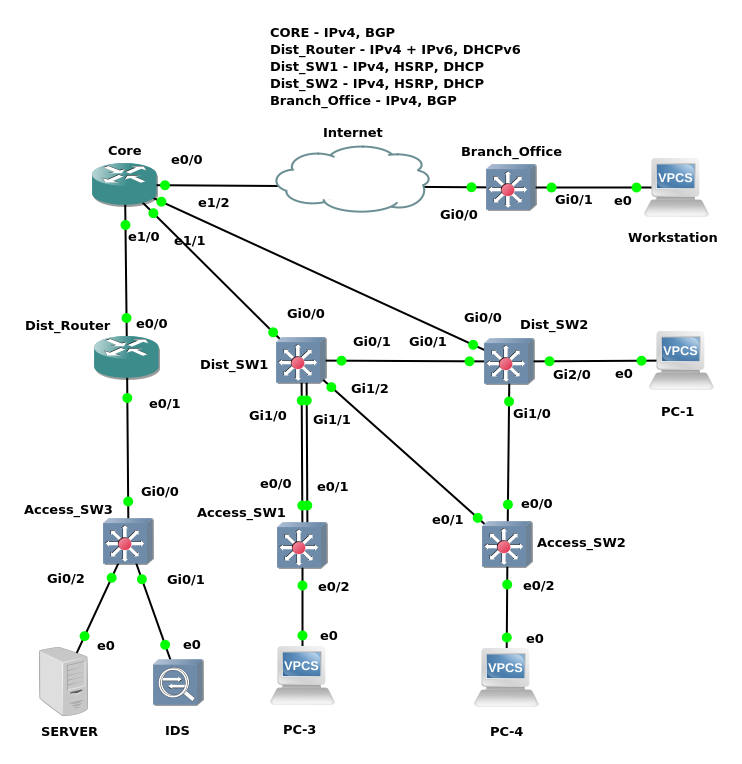
\includegraphics[scale=0.6]{obrazky/gns_topologia.png}
	\end{center}
	\caption[Testovacia topológia, pre ktorú sú dostupné vyexportované nastavenia zariadení.]{Testovacia topológia, pre ktorú sú dostupné vyexportované nastavenia zariadení.}
	\label{gns_topology}
\end{figure}



